\begin{figure}
\begin{ccTexOnly}
\begin{center}
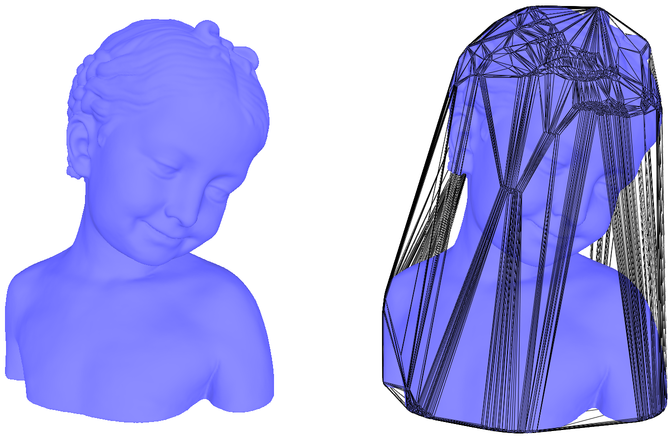
\includegraphics[width=12cm]{Convex_hull_3/chull_bimba.png}
\end{center}
\end{ccTexOnly}
\begin{ccHtmlOnly}
<CENTER>
<img border=0 src="./chull_bimba.png" alt="the convex hull of the bimba model">
</CENTER>
\end{ccHtmlOnly}
\caption{The convex hull of a model made of 192135 points.
\label{fig-ch-bimba}}
\end{figure}

\section{Introduction}

A subset $S \subseteq \R^3$ is convex if for any two points $p$ and $q$
in the set the line segment with endpoints $p$ and $q$ is contained
in $S$. The convex hull of a set $S$ 
is the smallest convex set containing
$S$. The convex hull of a set of points $P \in \R^3$ is a convex 
polytope with vertices in $P$. A point in $P$ is an extreme point 
(with respect to $P$) if it is a vertex of 
the convex hull of $P$.  A set of points is said to be strongly convex %
\ccIndexMainItemDef{strongly convex} if it consists of only extreme points.

This chapter describes the functions provided in
\cgal\ for producing convex hulls in three dimensions as well as
functions for checking if sets of points are strongly convex are not.  
One can compute the convex hull of a set of points in three dimensions
in one of three ways in \cgal: using a static algorithm,
using an incremental construction algorithm, or using a
triangulation to get a fully dynamic computation.

